\chapter{Experimental Analysis and Results}
\label{ch:results}

This chapter presents an analysis of effort from traditional procedures to the use of \textit{Sesnando} and an anslysis of the capability of this tool. It also presents an analysis of requirement complexity and how \textit{Sesnando} deals with them. \textcolor{red}{reforçar}

\section{Effort analysis}
%----------------------- Effort Analysis ----------------------------
\label{subsec:results_effor_analysis}

This section presents the obtained results using the traditional methods versus the obtained results using the \textit{Sesnando} application. The results presented here were applied on a real railway project for a rolling stock manufacturer.

In order to write system test specifications for such project, several steps are required, these steps are illustrated on Figure \ref{fig:traditional_method}. First, new requirements need to be obtained from the Requirement management tool such as IBM Doors, the software under testing needs to be downloaded or the remote test racks needs to be accessed depending on the nature of the requirement, SIL0 or SIL2 respectively (See Section \ref{sec:current_procedures}).\\

The designing of a test specification requires the identification of the applicable software signals on the Interface Control Document (ICD), as defined on section \ref{sec:current_procedures} that satisfy the conditions of those requirements. As well as software signals, the requirement clauses need to be identified and combined according to the applicable requirement coverage criteria in the in the form of test steps. Once all \textit{Test Requirements} are identified, the tester must generate a test script, which is generated by a VBA program and is then run against the current software release and a test report is automatically generated by the manufacturer test tool once the test finishes. Figure \ref{fig:system_test_spec} presents a manually written test specification using traditional procedures.

\begin{figure}[h]
    \centering
    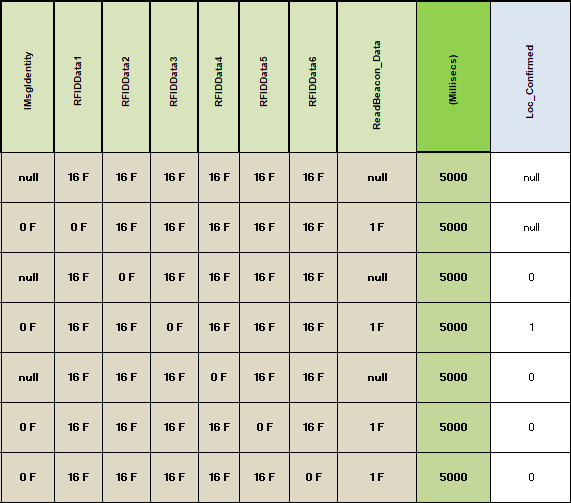
\includegraphics[width=\textwidth]{images/traditional_test_spec.PNG}
    \caption{System test specification - Traditional method}
    \label{fig:system_test_spec}
\end{figure}

The design of a test specification using traditional method results on test tables similar to Figure \ref{fig:system_test_spec}. The columns represent the signal values to be set on the target system and in purple, the expected signals, or in other words, the outcome of the test step. The content of this test specification is not really important for the subject. The main idea is to demonstrate that \textit{Sesnando} is able to generate similar test specifications as presented on Section \ref{subsec:test_generation}.\\

Both the test specification and test report (which is an HTML file generated by the manufacturer test tool discriminating all pass/fails for every test step) 

are subject to a peer review. The goal of this activity is to detect possible human errors and validate the test results if no flaws are detected. An introduced human error on the specification will influence the test results, as such, the specification needs to be redesigned and re-executed.\\

\begin{figure}[p]
    \centering
    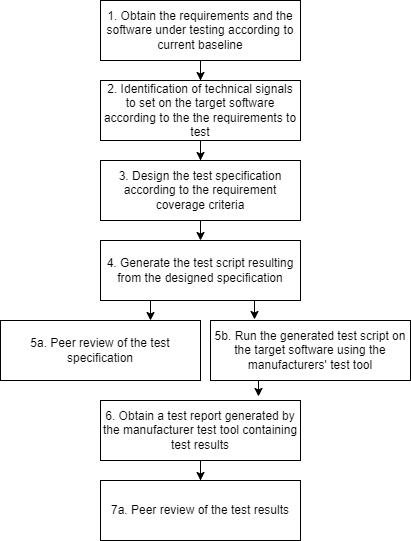
\includegraphics[scale=0.9]{images/traditional_methods.png}
    \caption{Traditional methods core steps}
    \label{fig:traditional_method}
\end{figure}

\textit{Sesnando} significantly reduces the effort involved in this process by automating the activities involved on steps 2. and 3. of Figure \ref{fig:traditional_method}, this results in the diagram of Figure \ref{fig:sesnando_method}, in other words, by automatically generating the test specification containing all the test steps, input and output signals (expected results). The requirements of the railway project must be loaded to \textit{Sesnando} which then connects to a remote service (Signal Manager) to acquire the corresponding software signals (this process is automatic). Once done, it will automatically generate a set of test steps using the project requirement coverage criteria and returns a test script compatible with the manufacturer test tool. The activity of peer reviewing should not be discarded, as human errors might be introduced on software signals repository.\\

\begin{figure}[p]
    \centering
    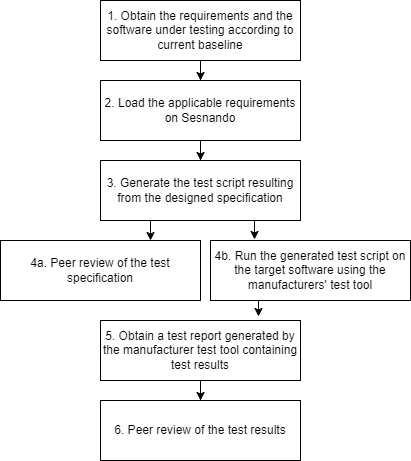
\includegraphics[scale=0.9]{images/sesnando_methods.png}
    \caption{Testing activities using Sesnando}
    \label{fig:sesnando_method}
\end{figure}

\textcolor{blue}{incluir um diagrama com os passos acima definidos}

A research was carried out at CSW to accurately determine the effectiveness of \textit{Sesnando}. Four people were inquired for the spent effort to design a test specification for a single requirement. Given that the most common activities between \textit{Sesnando} and manual procedures are the technical signal identification and test generation, those will be considered for comparison.\\

Table \ref{tab:effort_manual_testing} illustrates the effort that each participant (identified as P1 to P4) took to determine the software technical signals for a given requirement and the writing of the specification. They've all worked on the same requirement.

\begin{table}[h]
\caption{Effort using traditional methods}
    \footnotesize
    \centering
    
    \begin{tabular}{c c c}
        \hline
        % --- ROW Header --- %
        \textbf{\textit{Participant}} & 
        \textbf{\textit{Technical Signal Analysis}} & 
        \textbf{\textit{Specification Writing}}\\ \hline  \\
        
        % --- ROW 1 --- %
        \begin{tabular}[c]{@{}c@{}} \textbf{\textit{ P1 }} \end{tabular} & 
        15 Min. & 
        75 Min. \\
        \hline \\
        
        % --- ROW 2 --- %
        \begin{tabular}[c]{@{}c@{}} \textbf{\textit{ P2 }} \end{tabular} & 
        15 Min. &
        120 Min. \\
        \hline \\
       
        % --- ROW 3 --- %
        \begin{tabular}[c]{@{}c@{}} \textbf{\textit{ P3 }} \end{tabular} & 
        45 Min. &
        195 Min. \\
        \hline \\
        
        % --- ROW 4 --- %
        \begin{tabular}[c]{@{}c@{}} \textbf{\textit{ P4 }} \end{tabular} & 
        30 Min. &
        105 Min. \\
        \hline \\
        
         % --- ROW 5 --- %
        \begin{tabular}[c]{@{}c@{}} \textbf{\textit{ Avg. P}} \end{tabular} & 
        \textbf{26 Min.} &
        \textbf{123 Min.} \\
        \hline \\
        
    \end{tabular}
    \label{tab:effort_manual_testing}
\end{table}

Taking the results obtained from the participants, Technical signal analysis represents an average effort of 26 minutes and the writing of the specification represents an average effort of 123 minutes for a single requirements containing a couple of AND conditions, resulting on an average of approximately \~ 250 minutes per simple requirement. A participant also stressed out that most complex requirements can take up to two days to have a specification ready.

\textit{Sesnando} is able to reduce the effort needed for both activities mentioned on \ref{tab:effort_manual_testing} for less that 1 minute, as through a simple application launch results in a generated specification. When using \textit{Sesnando}, the requirement signals need to be available on the \textit{Signal Manager}. The ideal scenario would be to have all the necessary signals on the \textit{Signal Manager}, so a specification is generated for any given requirement instantly. At the current stage of development, a functionality is being created, so ICDs and Input signal Documents can be uploaded to populate the remote Signal Manager Repository \ref{sec:functional_overview}, as every tester will benefit from this. However, adding signals manually is already possible.\\

It is important to enumerate the scenarios where Requirement signals are not available on the remote tool. The participants were asked to add a couple of signals to the Signal Manager. The effort required to generate a specification using \textit{Sesnando} is determined as on Table \ref{tab:effort_auto_testing}.
The Signal Manager is now referenced as SM.

\begin{table}[h]
\caption{Effort using Sesnando}
    \footnotesize
    \centering
    
    \begin{tabular}{c c c}
        \hline
        % --- ROW Header --- %
        \textbf{\textit{Scenario}} & 
        \textbf{\textit{Technical Signal Analysis}} & 
        \textbf{\textit{Specification Writing}}\\ \hline  \\
        
        % --- ROW 1 --- %
        \begin{tabular}[c]{@{}c@{}} 
            \makecell{
                \textbf{\textit{ Existing Signals }} \\
                \textbf{\textit{ on Signal Manager }} \\ 
                \textbf{\textit{ (Best Case Scenario) }}
            }
        \end{tabular} & 
        < 1 min. & 
        < 1 min. \\
        \hline \\
        
        % --- ROW 2 --- %
        \begin{tabular}[c]{@{}c@{}} 
        \makecell{\textbf{\textit{ Signals not available }} \\ \textbf{\textit{ Experienced user in SM }}} 
        \end{tabular} & 
        ~10 Min. &
        < 1 min. \\
        \hline \\
       
        % --- ROW 3 --- %
        \begin{tabular}[c]{@{}c@{}}
        \makecell{\textbf{\textit{ Signals not available }} \\ \textbf{\textit{ Unexperienced user in SM }} \\ \textbf{\textit{ (Worst Case Scenario) }}
        }
        \end{tabular} & 
        25-35 Min. &
        < 1 min. \\
        \hline \\
        
    \end{tabular}
    \label{tab:effort_auto_testing}
\end{table}


On the worst case scenario a tester needs to identify technical signals on the available project resources, such as ICDs, learn how to use the Signal Manager and insert the found technical signals to be used by \textit{Sesnando} in the future. However the generation of the specification is always instant.
During this process it shall be considered the time that each participant took to learn the tool (\textit{Px(Technical Signal Analysis) + Learning SM + Adding signals}). This process is not applicable for future requirements that use the same signals, as the will already be available. According to obtained results, \textit{Sesnando} can save up to 90\% of effort spent during the system testing activities.\\

\section{Requirement complexity analysis}
%----------------------- Complexity Analysis ----------------------------
\label{subsec:results_req_complexity}

This section presents an analysis of complexity of requirements, how \textit{Sesnando} interprets them and what were the difficulties on this process.

To analyse the complexity of existing requirements a set of eighty (80) requirements has been exported and for each one, a value of 1 to 4 was assigned. The result of this analysis is shown on Table \ref{tab:req_complexity_analysis}.

\begin{table}[H]
\caption{Requirement Complexity Analysis}
    \footnotesize
    \centering
    
    \begin{tabular}{c c c}
        \hline
        % --- ROW Header --- %
        \textbf{\textit{Complexity}} & 
        \textbf{\textit{Number of Req.}} & 
        \textbf{\textit{Req. Percentage}}\\ \hline  \\
        
        % --- ROW 1 --- %
        \begin{tabular}[c]{@{}c@{}} \textbf{\textit{ 1 - Interpretable }} \end{tabular} & 
        22 & 
        27\% \\
        \hline \\
        
        % --- ROW 2 --- %
        \begin{tabular}[c]{@{}c@{}} \textbf{\textit{ 2 - Requires Rewrite }} \end{tabular} & 
        13 &
        17\% \\
        \hline \\
       
        % --- ROW 3 --- %
        \begin{tabular}[c]{@{}c@{}} \textbf{\textit{ 3 - Tool to be improved }} \end{tabular} & 
        29 &
        37\% \\
        \hline \\
        
        % --- ROW 4 --- %
        \begin{tabular}[c]{@{}c@{}} \textbf{\textit{ 4 - Non-Compatible }} \end{tabular} & 
        15 &
        19\% \\
        \hline \\
        
        
    \end{tabular}
    \label{tab:req_complexity_analysis}
\end{table}

The Complexity analysis was applied to the existing requirements and measured from 1 to 4, the description of each complexity level is described as follows:
\begin{itemize}
\item 1 - Interpretable - The existing requirement is written in a way that is already interpretable by \textit{Sesnando} and its test specification can be generated.
\item 2 - Requires rewrite - The existing requirement is malformed or contains words, characters or expressions that are not interpretable by \textit{Sesnando}, however, its main logic is supported after the rewriting of such requirement.
\item 3 - Tool to be improved - The existing requirement contains expressions that needs additional checkings like signal pulses or depend on the output of other existing requirements.
\item 4 - Non-Compatible - Requirements that require more than a signal observation or information that is out-of-scope of \textit{Sesnando}, usually, those are defined as semi-automated tests and require a manual action from the tester.
\end{itemize}

This analysis concludes that from the selected sample of requirements 27\% of the existing requirements can be interpreted by \textit{Sesnando}, 17\% are not compliant with the predefined grammar and need rewriting, 37\% of the requirements requires new developments on \textit{Sesnando} as they require specific observations e.g. a signal value is set within a given timeframe, 19\% or requirements cannot be handled by \textit{Sesnando} as they cannot be verified solely on signal analysis and require the observation of the tester e.g. an icon is blinking on the drivers' desk (on traditional methods, these are semi-automated tests).





